\documentclass{article}
\usepackage{../../pset}

\lhead{6.832 Proposal}
\chead{}

\renewcommand\labelitemi{--}

\begin{document}
\begin{center}
	\huge
	Inverted Double Pendulum
\end{center}

\section{Introduction}

The double pendulum is a classical system with complex mechanics. However, the underactuated system with a single actuator at the shoulder can still stabilize in the inverted position as in \cref{fig:inverted_double_pendulum}.

For this project, I will build the physical plant with the necessary sensors and actuators, construct and tune a energy-shaping and LQR controller, and use the actuator to stabilize the system in the upright position.

This project is worthwhile to grasp the challenges of building and designing control for a physical system. There is benefit to putting everything in action first on a simple pendulum. The real fun will come when formulating the control for the double pendulum, which is more complex than anything we've implemented on the psets so far.

I am doing this project jointly for 6.832 and 6.115 (Microcontroller Lab).

\begin{figure}[h]
	\centering
	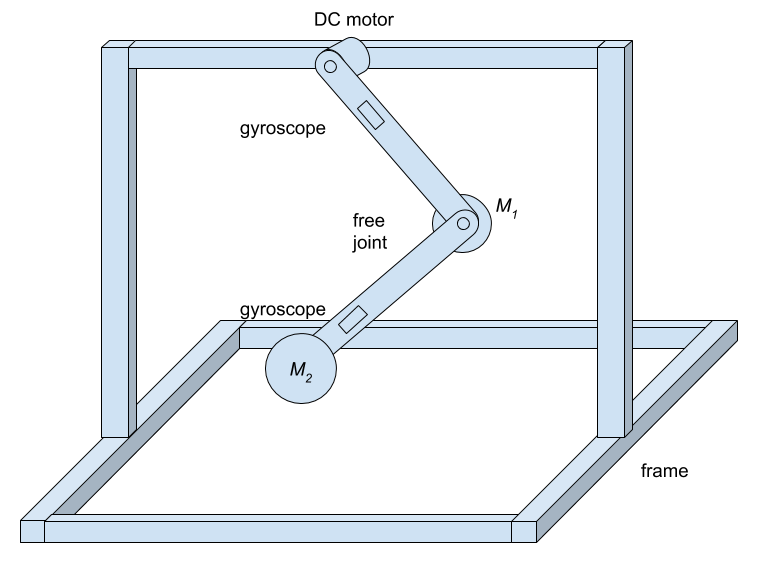
\includegraphics[width=4in]{double_pendulum.png}
	\caption{Double pendulum with single actuator at the top.}
	\label{fig:double_pendulum}
\end{figure}

\begin{figure}[h]
	\centering
	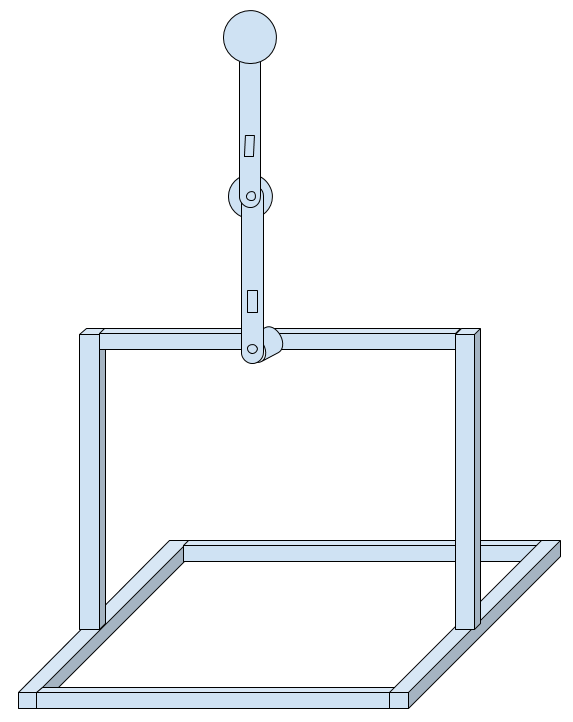
\includegraphics[width=3in]{inverted_double_pendulum.png}
	\caption{Inverted double pendulum.}
	\label{fig:inverted_double_pendulum}
\end{figure}

\section{Implementation Description}

The two gyroscope sensors communicate to the microcontroller. The angles and angular velocities of the two arms completely determine the state of the physical system at any point in time. The microcontroller uses these quantities to compute the torque that the motor should apply and will use PWM to power the DC motor.

As in pset 3, the controller will have two modes. The first is the energy-shaping controller, which tries to give the system the right amount of energy (while keeping the angular velocities low). Once the system reaches the region of convergence, the controller will switch to using a Linear Quadratic Regulator to stabilize the pendulum at its peak.

\section{Project Scope and Management}
Before attempting with a double pendulum, I will make sure I can work with a single pendulum (using just the first arm). The energy-shaping controller and LQR controller can be implemented, tested, and demonstrated separately.

Simultaneously with that, I will make sure that I can control the inverted double pendulum in pydrake simulation.

Once these parts are working, I will add the second arm to to the physical system and try the new controller.

\section{Timeline}
Week of 4/16:
\begin{itemize}
	\item Build the frame and cut parts
	\item Run an LQR and energy-shaping controller in pydrake
\end{itemize}
Week of 4/23:
\begin{itemize}
	\item Program the microcontroller to apply PWM with a variable duty cycle
	\item Play with gyroscope sensors
	\item Finish building plant
\end{itemize}
Week of 4/30:
\begin{itemize}
	\item Implement LQR controller for single pendulum on the microcontroller
	\item Implement energy-shaping controller on the microcontroller
	\item Calculate the region of convergence for LQR
	\item System should work fully on single pendulum
\end{itemize}
Week of 5/7:
\begin{itemize}
	\item Attach second arm
	\item Update controllers for double pendulum dynamics
	\item System should work fully on double pendulum
\end{itemize}
Week of 5/14:
\begin{itemize}
	\item Test with counterforces
	\item Reduce available power
	\item Make control smooth and robust
	\item Finish writing report
\end{itemize}

\end{document}
